This chapter covers the implementation of the text-aware process prediction model presented in the previous chapter.
In Section \ref{sec:technology} the underlying technology is depicted, whereas in Section \ref{sec:model-implementation} the architecture of the implementation is defined.

\section{Technology}\label{sec:technology}

The implementation of the text-aware process prediction model is purely based on Python 3.6 \cite{python}.
The set of Python packages that are utilized for the implementation are summarized in Table \ref{tab:packages}.
All packages follow the open-source development model and are mostly community-driven.

\begin{table}[!htbp]
	\begin{tabularx}{\textwidth}{l p{4.5cm} p{6.6cm} }
		\toprule
		\textbf{Package} & \textbf{Developer(s)} & \textbf{Purpose}  \\
		\midrule
		PM4Py \cite{DBLP:journals/corr/abs-1905-06169}   &  Fraunhofer Institute for Applied Information Technology &  Event log parsing and handling\\
		TensorFlow \cite{DBLP:journals/corr/AbadiABBCCCDDDG16} &  Google Brain Team et al.& Construction and training of LSTM model \\
		NTLK \cite{DBLP:books/daglib/0022921} & Bird et al. & Text preprocessing\\
		Scikit-learn \cite{DBLP:journals/jmlr/PedregosaVGMTGBPWDVPCBPD11} & Cournapeau et al.& Bag of Words and Bag of N-Gram tf-idf encoding \\
		Gensim \cite{rehurek_lrec} & Řehůřek et al. & Latent Dirichlet Allocation and Paragraph Vector encoding \\
		 \bottomrule
	\end{tabularx}
	\caption[List of Python packages used for implementation]{List of Python packages used for implementation.}
	\label{tab:packages}
\end{table}

PM4Py \cite{DBLP:journals/corr/abs-1905-06169} is a Python package developed by the Fraunhofer Institute for Applied Information Technology, which offers a wide range of process mining algorithms and event log operations for the Python environment.
It is used for event log parsing and its internal event log representation.

TensorFlow \cite{DBLP:journals/corr/AbadiABBCCCDDDG16} is a dataflow oriented framework originally developed by Google, which includes a diverse set of neural network models and serves with its LSTM implementation using the Keras API \cite{chollet2015keras}.

Furthermore, the packages NTLK \cite{DBLP:books/daglib/0022921}, Scikit-learn \cite{DBLP:journals/jmlr/PedregosaVGMTGBPWDVPCBPD11} and Gensim \cite{rehurek_lrec} are applied for the preprocessing and encoding of textual data.
NTLK is used to realize the tokenization and word lemmatization, whereas the implementation of the text models is supported by the Scikit-learn (Bag of Words, Bag of N-Gram) and Gensim (LDA, Paragraph Vector) packages.


\section{Model Implementation}\label{sec:model-implementation}

The interface of the text-aware process prediction model (tapp) is realized through a class \texttt{TappModel}, which implements the functions \texttt{fit()},  \texttt{predict()} and  \texttt{evaluate()}, that can be used to fit the model to an event log with historical data, compute prediction for an event log with uncompleted traces and evaluate the performance of the prediction model.
The \texttt{TappModel} manages the underlying LSTM model and can be configured with the number of shared and specialized layers as well as the dimension of the hidden neurons per LSTM layer.

\begin{figure}[htbp!]
	\centering
	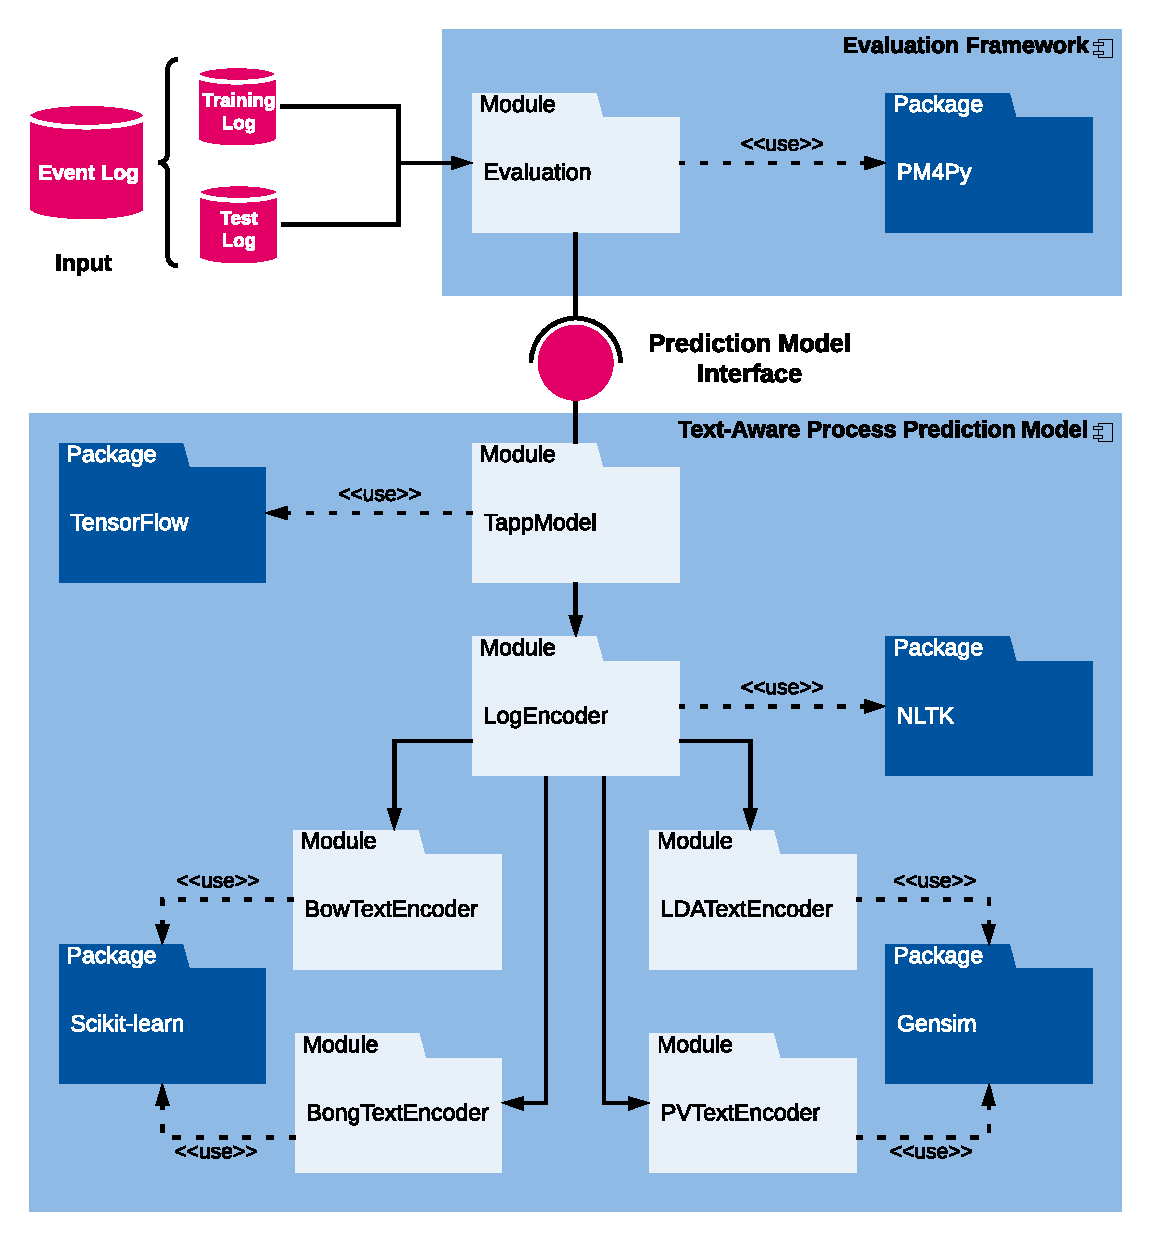
\includegraphics[width=\textwidth]{figures/implementation}
	\caption[Component diagram of the implementation]{Component diagram of the implementation.}
	\label{fig:/implementation}
\end{figure}

The encoding of traces as described in Section \ref{sec:event}, \ref{sec:time} and \ref{sec:text} is computed in the \texttt{LogEncoder} module, which is controlled by the \texttt{TappModel}.
The \texttt{LogEncoder} is also fitted to the historical log and can transform (prefix) traces to the encoded matrix format via functions \texttt{fit()} and \texttt{transform()}.
It is configured with one out of the four text encoding models described in Section \ref{sec:text} (\texttt{BowTextEncoder},  \texttt{BongTextEncoder}, \texttt{LDATextEncoder} and  \texttt{PVTextEncoder}), that realizes the vectorization of textual data.
Just like the \texttt{LogEncoder}, the text encoding models offers the functions \texttt{fit()} and \texttt{transform()} adapt to the historical data and compute the text encoding.

During the fitting phase of the  \texttt{LogEncoder}, all possible values for categorical attribute are indexed and the parameters for the normalization of numerical attributes are computed.
With regard to the text encoding model, the indexed vocabulary of all words (after preprocessing) in the historical event log is built during fitting.
In case of the Paragraph Vector model, the encoding network is trained with the training corpus.

The text-aware process prediction model can be used in any business process monitoring software to provide the prediction capabilities using the methods of the \texttt{TappModel}.
In order to evaluate the performance of the model, an experiment using the \texttt{Evaluation} module is performed, which is described in-depth in Chapter \ref{chap:eval}.
The module reads an event log using PM4Py, divides it into a training and test log and measures the prediction performance of differently configured instances of the text-aware process prediction model.
An overview of the different components of the implementation is shown in Figure \ref{fig:/implementation}.